
\chapter{Point de Situation}
\label{chap:choix}

\section{Contexte}
La première partie du projet nous a permis de redéfinir le sujet et les attentes, mais également de réfléchir aux solutions technologiques que nous pourrions utiliser. Après avoir observé les solutions existantes et compte tenu du budget qui nous est imposé, la solution générale retenue sera donc la suivante: les ondes radio captées par les antennes, seront traitées par un filtre et un down-converter avant de passer par le radiogoniomètre et obtenir une position angulaire qui sera envoyée au serveur puis transmise à l’IHM (voir dans le chapitre \ref{chap:choix} la partie \ref{sec:phys}).

Cependant, de nombreuses zones d’ombres planent encore sur la réalisation technique, notamment car nous ne maitrisons pas le domaine. En effet, nous utiliserons des plans de carte électronique de radiogoniomètre amateur afin de réaliser notre solution technologique, car réaliser un traitement entièrement numérique ne semble pas réalisable dans le temps impartit. 

De plus, actuellement, nous ne nous sommes pas encore réellement penchés sur le traitement des informations ainsi que sur la structure du serveur et de l’IHM. Nous avons seulement convenu que le transfert des informations se fera via Arduino. L’un d’entre eux sera le serveur et dialoguera avec l’ensemble des autres Arduino positionnés sur les antennes.~\\


Actuellement, nous ne possédons aucune partie physique du projet et nous réalisons des listes de commandes afin de pouvoir commencer les tests unitaires le plus rapidement possible.

\section{Rappel de notre projet}

Suite à notre état de l'art, nous avons décidé de réaliser notre système de détection en installant un maillage de capteur qui se baseront sur le système du Montréal 3V2. Chaque capteur sera connecté à un \rpi 2 \footnote{La documentation technique du Raspberry PI est situé en annexe à la page \pageref{annexe:rpi}}. De plus, chaque \rpi communiquera avec un ordinateur central qui traitera les données pour les afficher sur une interface graphique. Les données qui seront transmises sont: le numéro du \rpi, la position du capteur, et le gisement du drone par rapport au capteur. Enfin, l'ordinateur central communiquera avec une application android qui notifiera le client de la présence d'un drone comme on peut le voir sur la figure \ref{fig:inst}.
~\\

\begin{figure}[!h]
  \centering
  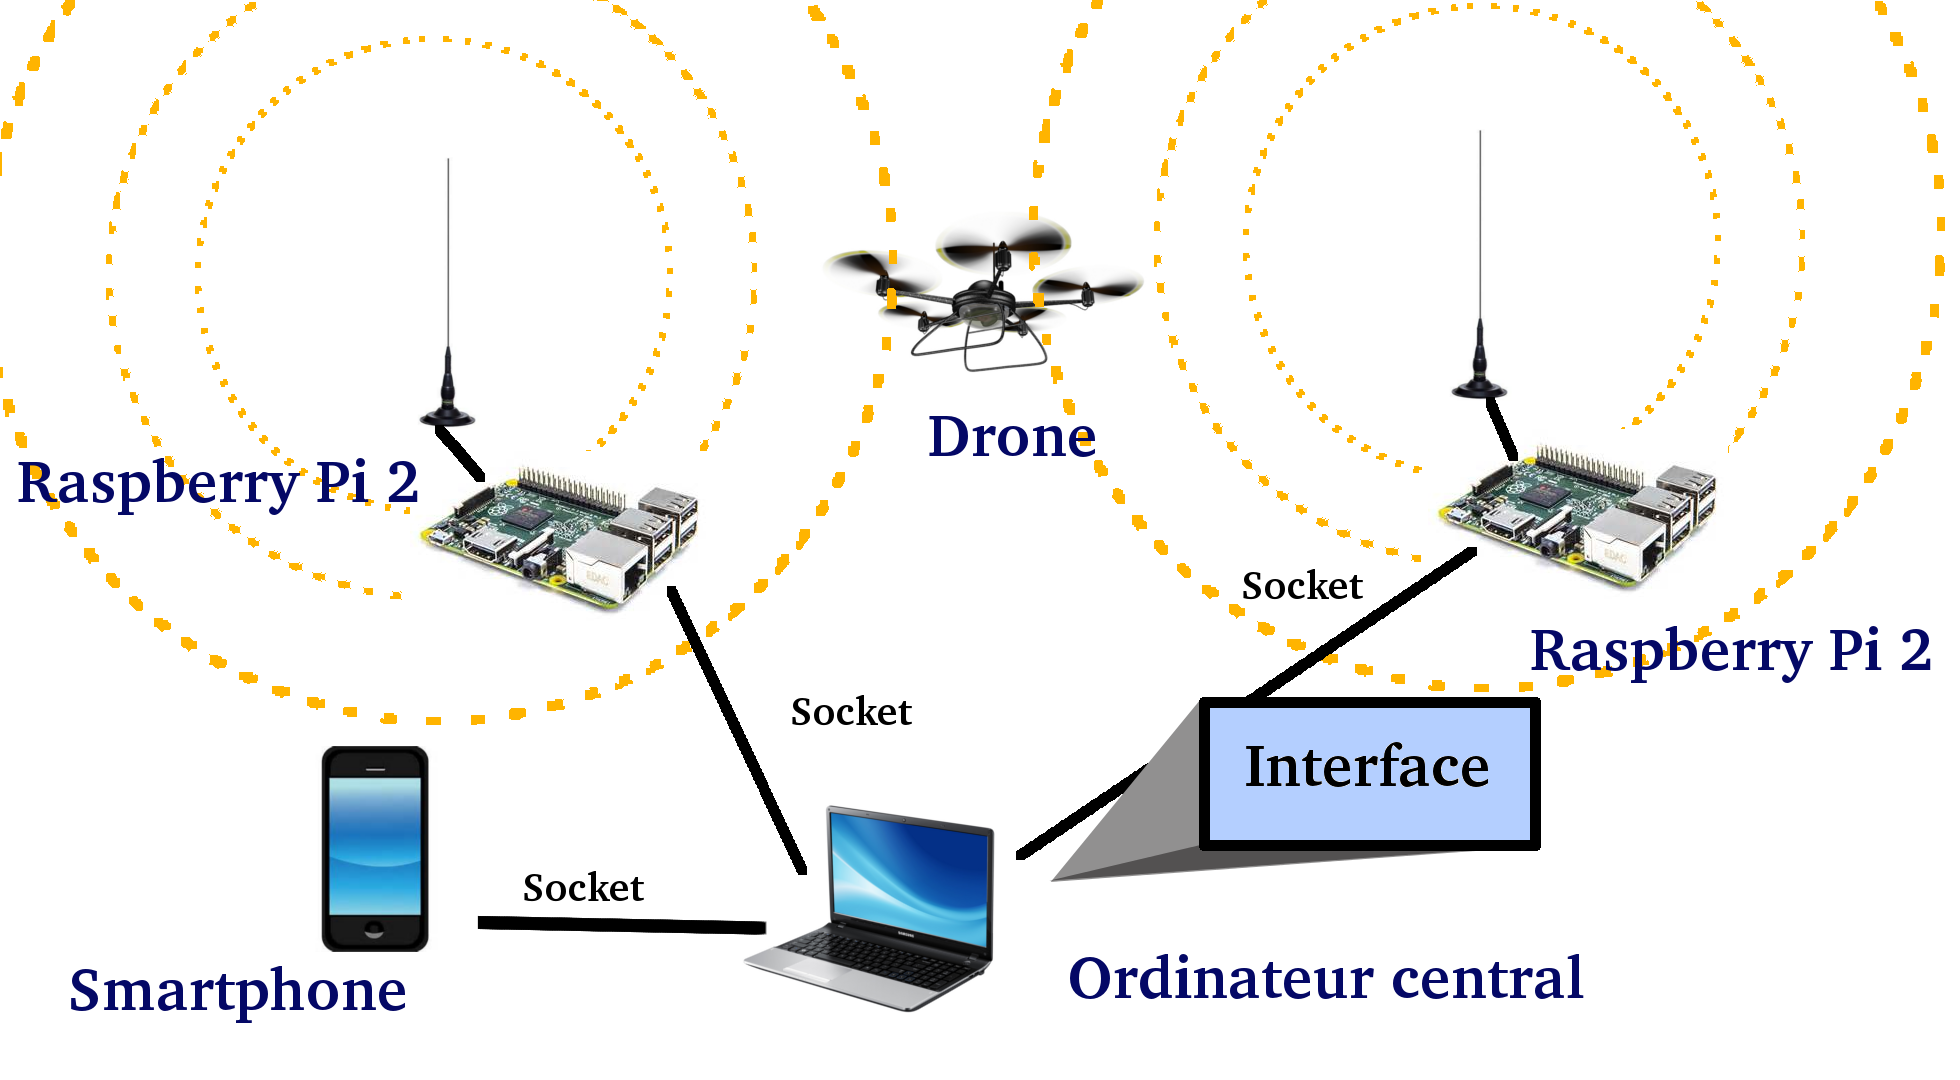
\includegraphics[width=\textwidth]{installation}
  \caption{Installation de Smart}
  \label{fig:inst}
\end{figure}


\section{Architecture Fonctionnelle}
En début de projet, suite à l'interview de notre encadrant Mr. Ali Mansour, nous avions réalisé le tableau de exigence (tableau \ref{pdf:tab}).


L'ensemble de notre projet c'est donc construit autour de ces premières exigences, qui on ensuite été détaillées en fonctions et contraintes. Très vite, nous avons convenu que l'architecture fonctionnelle de notre système serait telle que décrite dans le diagramme SADT ci dessous.

\begin{figure}[h]
  \begin{minipage}{0.45\linewidth}
    \centering
    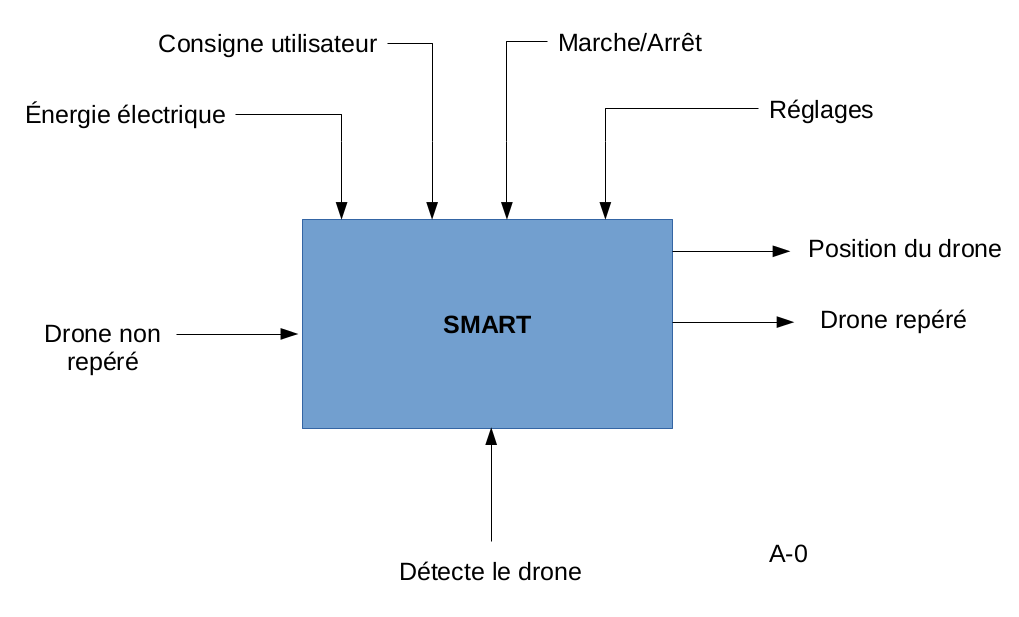
\includegraphics[width=\textwidth]{SADTA-0}
    \caption{SADT A-0}
  \end{minipage}\hfill
  \begin{minipage}{0.45\linewidth}
    \centering
    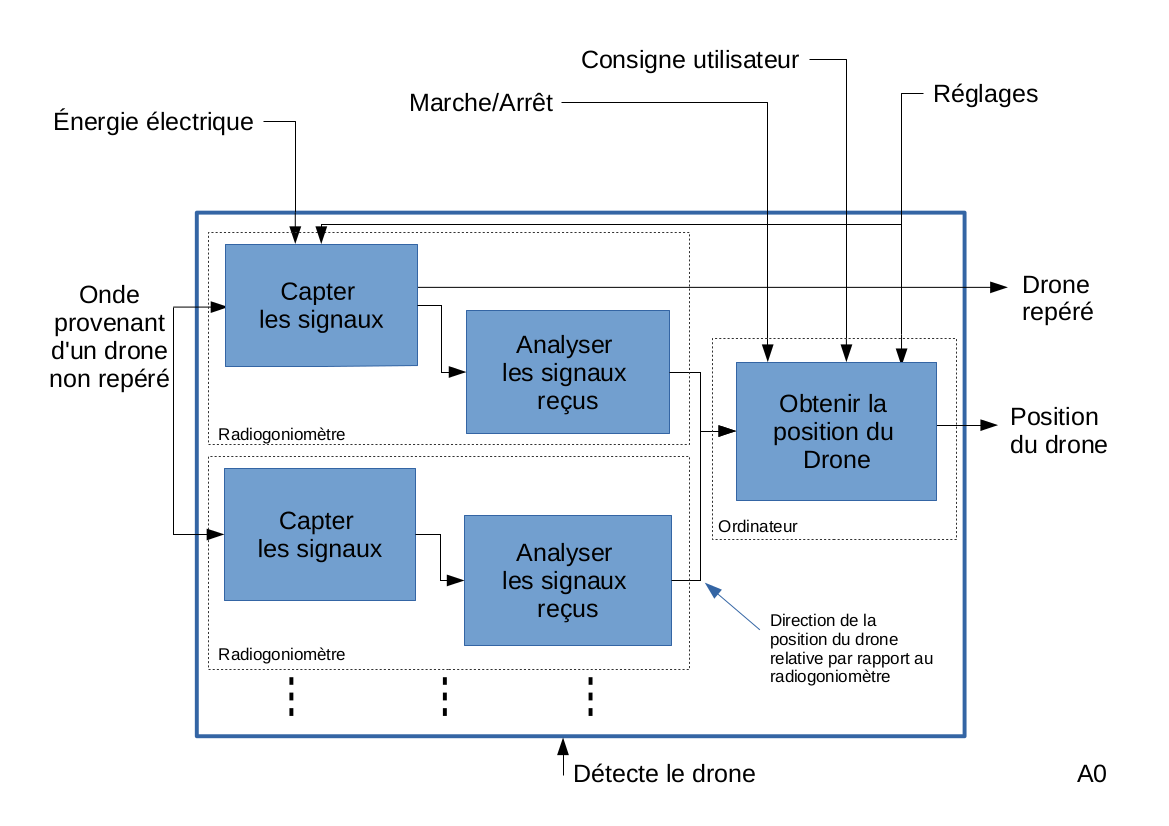
\includegraphics[width=\textwidth]{SADTA0}
    \caption{SADT A0}
  \end{minipage}
\end{figure}




Comme on peut le voir, le fonctionnement de notre système est décrit en trois grandes actions: 
\begin{itemize}
\item capter les signaux émis par une source inconnue en restant à l'écoute
\item analyser les signaux reçus et traiter ces derniers grâce à une succession de filtres
\item obtenir la position du drone par triangulation grâce aux angles de détection obtenus
\end{itemize}


\begin{figure}[h]
  \centering
  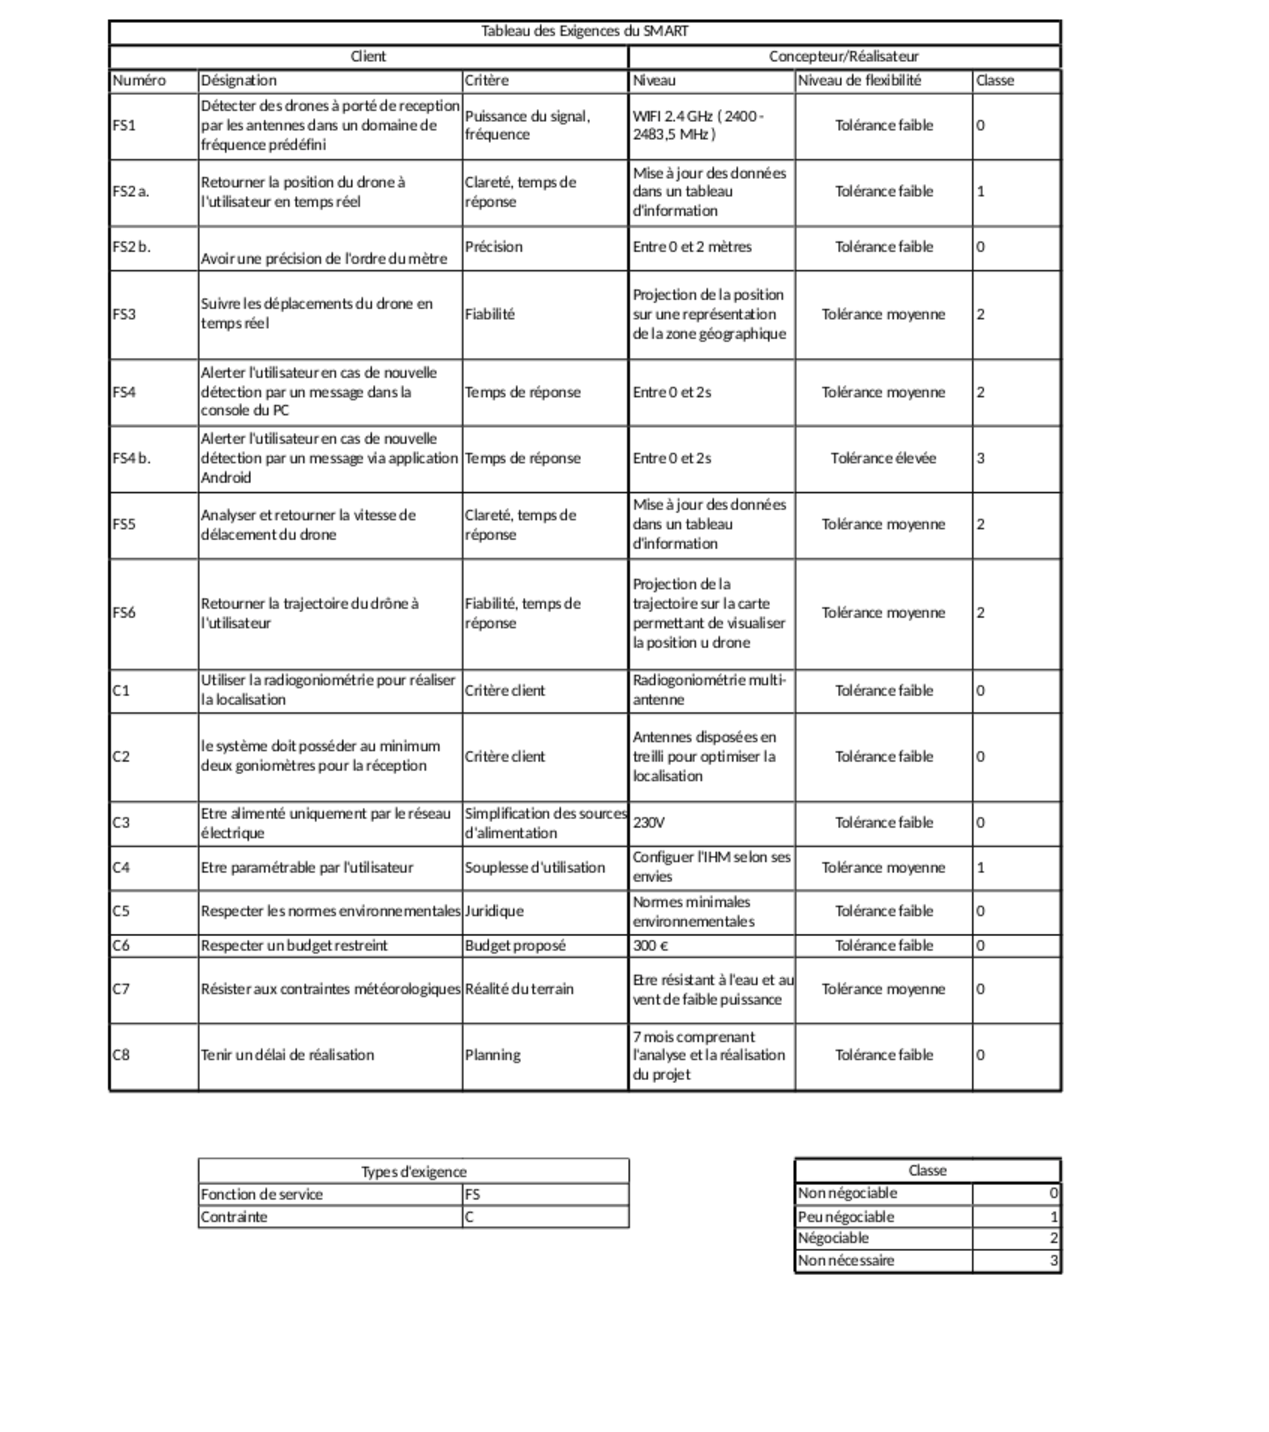
\includegraphics[width=\textwidth]{tableauSpe}
  \caption{Tableau des spécifications}
  \label{pdf:tab}
\end{figure}

 

\newpage


\section{Architecture physique}
\label{sec:phys}

Suite à l'analyse fonctionnelle nous avons avons fait le choix d'une architecture physique.
Pour cela nous avons découpé notre système en plusieurs sous-systèmes de la façon suivante:

\begin{figure}[h]
  \centering
  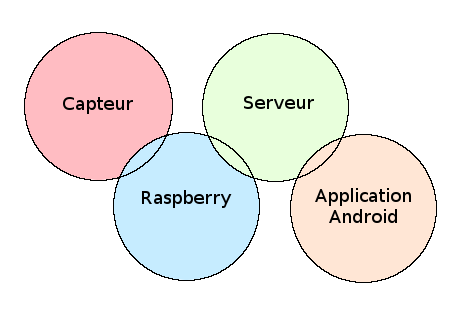
\includegraphics[width=0.8\textwidth]{SSysteme}
  \caption{sous-système}
\end{figure}

Tout d'abord, pour le capteur nous avons choisi de nous appuyer sur le Montréal 3v2 que nous avons choisi d'adapter à notre problème. Pour cela nous avons du adapter les antennes a nos fréquences, installer un filtre passe bas et enfin un down converter, mais nous avons garder le goniomètre du Montréal 3v2.

Ensuite, nous avons choisi de placer un petit ordinateur au niveau de chaque capteur qui servira de client TCP/IP transmettant ses informations à un ordinateur central. Pour répondre à ce besoin nous avons choisi d'installer des Raspberry Pi, pour des raisons évidentes de coût et de taille.

Puis nous avons choisi d'installer un ordinateur central (le serveur) rassemblant les données. Au cour de notre projet nous avons utilisé nos ordinateurs personnelles mais à termes nous souhaitons installer le serveur sur un Raspberry Pi.

Enfin, nous avons créé une application android fonctionnant sur nos téléphones personnels.


L'architecture physique du système est présenté à la figure \ref{fig:arch_phys}.

\begin{figure}[h]
  \centering
  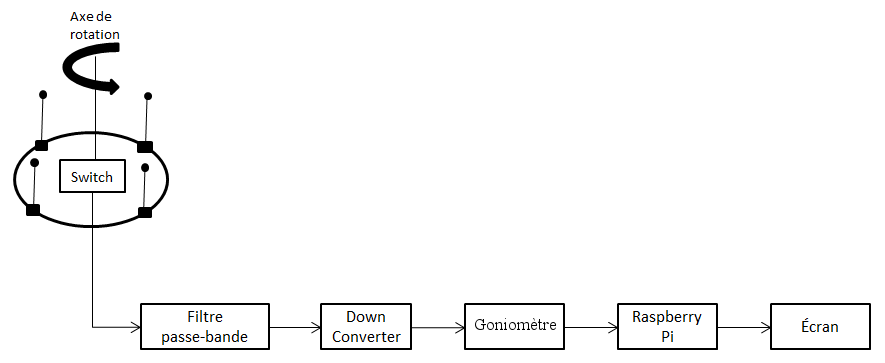
\includegraphics[width=\textwidth]{fonctionnement}
  \caption{Architecture Physique}
  \label{fig:arch_phys}
\end{figure}
\newpage

\newpage
\section{Treillis de détection}

Pour répondre au besoin de détection et s’assurer d’un correct positionnement de la cible, la mise en
place d’une couverture de détection répondant à nos besoins était nécessaire. Les critères retenus
pour cette dernière sont les suivants :

\begin{itemize}
\item A l’intérieur de la zone de détection, la cible doit être en permanence sous la couverture de détection de 4 radiogoniomètres
\item Tenter une optimisation de la couverture afin d’éviter l’installation d’un trop grand
nombre de radiogoniomètre
\end{itemize}

Très peu de sujets similaires ont pu être trouvé bien que le problème soit récurrent dans de
nombreux projets.

Cependant, après plusieurs essais, le choix de treillis fut le suivant :

\begin{minipage}{0.45\linewidth}

  \centering
  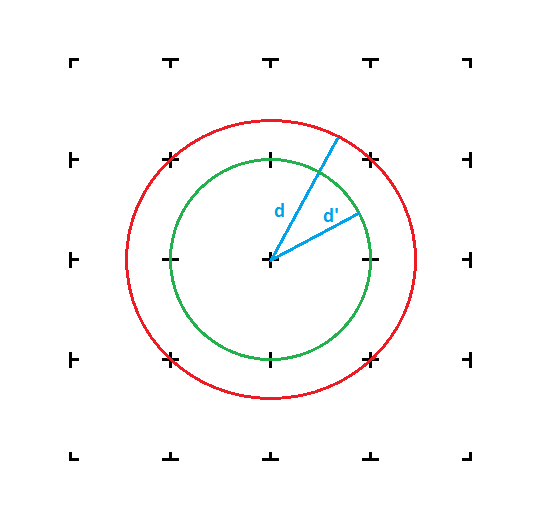
\includegraphics[width=\textwidth]{treillis_explication}
  \captionof{figure}{Cercle de détection}
  ~\\
\end{minipage}
\begin{minipage}{0.45\linewidth}
  \begin{itemize}
  \item Dans les deux cas, les distances d et d’ représente la distance de couverture maximale d’une antenne pour une configuration de treillis particulière, distance au-delà de laquelle nous ne sommes pas sûr d’assurer la détection d’un drone.
  \item Chaque croix noire représente une antenne. Ces dernières formes ainsi la zone de détection, zone à l’intérieure de laquelle, le drone se doit d’être repéré.
  \end{itemize}
\end{minipage}


Initialement, nous avions prévu que les antennes radiogoniométrique assureraient la détection
jusqu’à son plus proche voisin. Cependant, cette configuration ne permet pas d’assurer qu’un drone
traversant la zone soit sous la couverture d’au moins quatre antennes en tout temps. Nous avons
donc choisi la configuration représentée par le cercle rouge, c’est-à-dire en rapprochant les antennes
les unes des autres. On obtient ainsi la couverture suivante :
~\\

\begin{minipage}{0.45\linewidth}
  \centering
  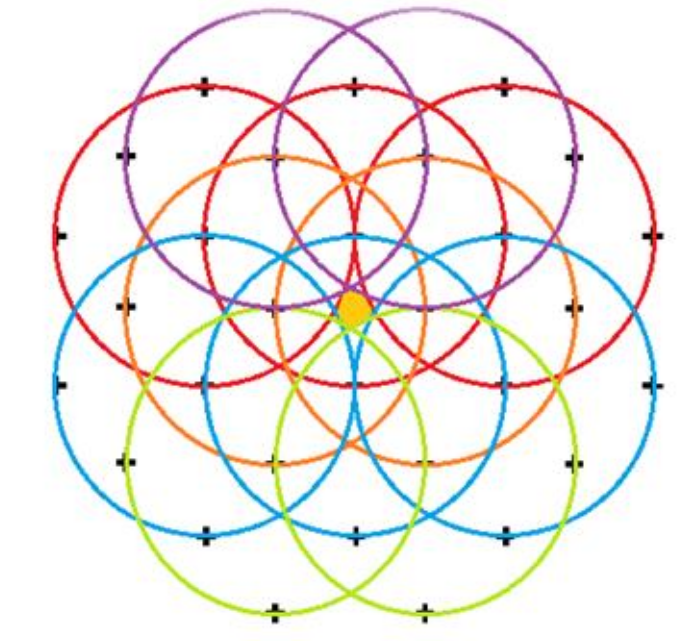
\includegraphics[width=\textwidth]{cercle}
  \captionof{figure}{Maillage de détection}
\end{minipage}
\begin{minipage}{0.45\linewidth}
  Dans cette configuration, les zones de plus faible couverture
sont situées sur les antennes elles même. En effet, au-dessus
de chaque antenne, la couverture n’est assurée que par
quatre d’entre elles. En dehors de celle-ci, la couverture est
assurée par cinq à six antennes.
\end{minipage}




%%% Local Variables: 
%%% mode: latex
%%% TeX-master: "../rapport"
%%% End: 
